\documentclass[12pt, a4paper]{article}
\usepackage{enumitem}
\usepackage{float}
\usepackage[left=2cm, right=2cm, top=2cm, bottom=2cm]{geometry}
\usepackage{graphicx}
\usepackage[colorlinks, urlcolor=blue]{hyperref}
\usepackage{minted}
\usepackage{xeCJK}

\renewcommand\arraystretch{1.1}
\setCJKmainfont[AutoFakeBold=1.5]{新細明體}
\setlength{\parindent}{0pt}

\setminted{
  frame=single,
}

\title{
  \vspace{-1cm}
  Network Administration/System Administration\\
  (NTU CSIE, Spring 2024)\\
  Homework \#8 - LDAP
}
\author{\Large B12902110 呂承諺}

\begin{document}
  \maketitle
  \section{Server Setup}
  \begin{enumerate}[label=(\alph*)]
    \item \textbf{LDIF files}

    \verb|suffix.ldif|
    \inputminted[fontsize=\footnotesize]{ldif}{ldif/suffix.ldif}

    \verb|root.ldif|
    \inputminted[fontsize=\footnotesize]{ldif}{ldif/root.ldif}

    \verb|records.ldif|
    \inputminted[fontsize=\footnotesize]{ldif}{ldif/records.ldif}

    \pagebreak
    \textbf{Steps}
    \begin{enumerate}[label=(\arabic*)]
      \item Install the packages.
      \begin{Verbatim}[frame=single]
$ apt install -y slapd ldap-utils
      \end{Verbatim}
      \item Modify the LDAP records.
      \begin{Verbatim}[frame=single]
$ ldapmodify -Y EXTERNAL -H ldapi:/// -f suffix.ldif
$ ldapmodify -Y EXTERNAL -H ldapi:/// -f root.ldif
$ ldapadd -D cn=admin,dc=nasa,dc=csie,dc=ntu -w admin \
    -H ldapi:/// -f records.ldif
      \end{Verbatim}
    \end{enumerate}

    \textbf{Result}
    \begin{Verbatim}[frame=single]
$ ldapsearch -x -b dc=nasa,dc=csie,dc=ntu
    \end{Verbatim}

    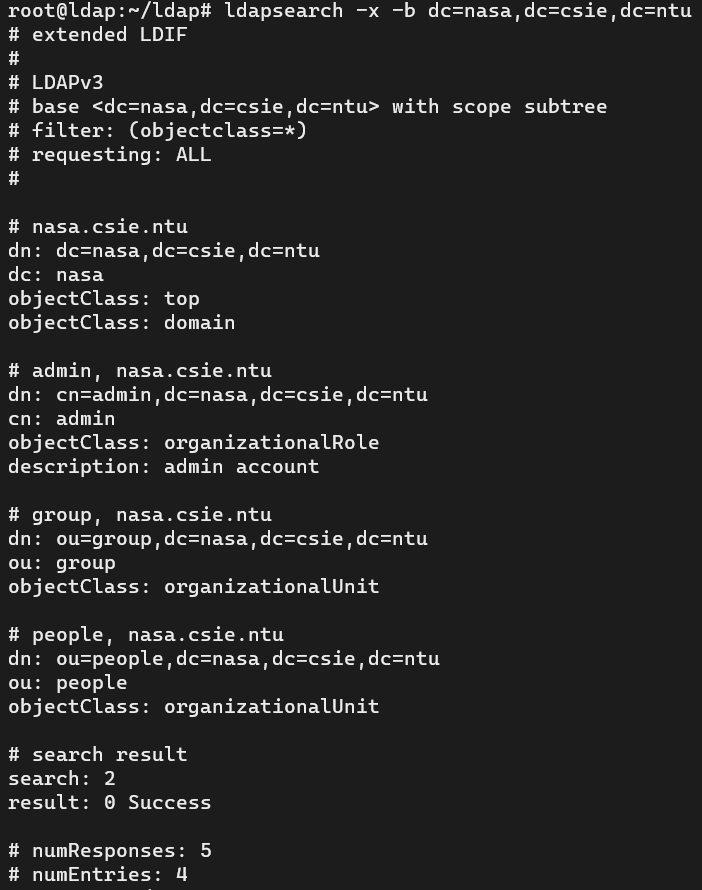
\includegraphics[width=0.7\textwidth]{1-a_ldapsearch.png}

    \textbf{References}
    \begin{itemize}
      \item \href{https://hackmd.io/@Mqvhsb9VRYSU2scAkRqGIQ/SJUufUTC6}{LDAP Lab - HackMD}
      \item \href{https://www.openldap.org/doc/admin26/slapdconf2.html}{OpenLDAP Software 2.6 Administrator's Guide: Configuring slapd}
    \end{itemize}

    \pagebreak
    \item \textbf{LDIF Files}

    \verb|tls_certificates.ldif|
    \inputminted{ldif}{ldif/tls_certificates.ldif}

    \textbf{Steps}
    \begin{enumerate}[label=(\arabic*)]
      \item Download script for generating certificates.
      \begin{Verbatim}[frame=single]
$ wget https://github.com/xbmc/openssl/raw/master/apps/CA.sh
$ chmod +x CA.sh
      \end{Verbatim}
      \item Generate CA certificate.
      \begin{Verbatim}[frame=single, fontsize=\footnotesize]
$ ./CA.sh -newca
CA certificate filename (or enter to create)

Making CA certificate ...

...

Check that the request matches the signature
Signature ok
Certificate Details:
        Serial Number:
            2a:49:2b:c0:1a:64:ca:46:81:3b:8d:cf:13:fb:ca:e8:30:bf:ae:e1
        Validity
            Not Before: Apr 27 18:40:57 2024 GMT
            Not After : Apr 27 18:40:57 2027 GMT
        Subject:
            countryName               = TW
            stateOrProvinceName       = Taiwan
            organizationName          = NTU CSIE
            commonName                = ca.nasa.csie.ntu
        X509v3 extensions:
            X509v3 Subject Key Identifier:
                54:37:93:4B:4E:C0:AA:16:F5:43:12:74:5E:23:AE:CD:30:AC:51:C8
            X509v3 Authority Key Identifier:
                54:37:93:4B:4E:C0:AA:16:F5:43:12:74:5E:23:AE:CD:30:AC:51:C8
            X509v3 Basic Constraints: critical
                CA:TRUE
Certificate is to be certified until Apr 27 18:40:57 2027 GMT (1095 days)

Write out database with 1 new entries
Database updated
      \end{Verbatim}

      \pagebreak
      \item Generate a certificate request.
      \begin{Verbatim}[frame=single, fontsize=\footnotesize]
$ ./CA.sh -newreq-nodes

...

Country Name (2 letter code) [AU]:TW
State or Province Name (full name) [Some-State]:Taiwan
Locality Name (eg, city) []:
Organization Name (eg, company) [Internet Widgits Pty Ltd]:NTU CSIE
Organizational Unit Name (eg, section) []:
Common Name (e.g. server FQDN or YOUR name) []:ldap
Email Address []:

...

Request (and private key) is in newreq.pem
      \end{Verbatim}

      \item Sign the certificate.
      \begin{Verbatim}[frame=single, fontsize=\footnotesize]
$ ./CA.sh -sign

...

Certificate Details:
        Serial Number:
            2a:49:2b:c0:1a:64:ca:46:81:3b:8d:cf:13:fb:ca:e8:30:bf:ae:e3
        Validity
            Not Before: Apr 27 19:43:08 2024 GMT
            Not After : Apr 27 19:43:08 2025 GMT
        Subject:
            countryName               = TW
            stateOrProvinceName       = Taiwan
            organizationName          = NTU CSIE
            commonName                = ldap
        X509v3 extensions:
            X509v3 Basic Constraints:
                CA:FALSE
            X509v3 Subject Key Identifier:
                56:48:59:6D:F1:53:E1:3D:19:40:5F:9B:52:BF:BA:CC:E6:E6:D3:D3
            X509v3 Authority Key Identifier:
                54:37:93:4B:4E:C0:AA:16:F5:43:12:74:5E:23:AE:CD:30:AC:51:C8
Certificate is to be certified until Apr 27 19:43:08 2025 GMT (365 days)
Sign the certificate? [y/n]:y

1 out of 1 certificate requests certified, commit? [y/n]y

...

Signed certificate is in newcert.pem
      \end{Verbatim}

      \item Copy the certificates to SLAPD's configuration folder, and set the
      file ownership and permission for \verb|serverkey.pem|.
      \begin{Verbatim}[frame=single]
$ cp demoCA/cacert.pem /etc/ldap/cacert.pem
$ mv newcert.pem /etc/ldap/servercrt.pem
$ mv newreq.pem /etc/ldap/serverkey.pem
$ chown openldap /etc/ldap/serverkey.pem
$ chgrp openldap /etc/ldap/serverkey.pem
$ chmod 600 /etc/ldap/serverkey.pem
      \end{Verbatim}

      \item Add the TLS certificate options to SLPD.
      \begin{Verbatim}[frame=single]
$ ldapmodify -Y EXTERNAL -H ldapi:/// -f tls_certificates.ldif
      \end{Verbatim}

      \item Change \verb|SLAPD_SERVICES| in \verb|/etc/default/slap|.
      \begin{Verbatim}[frame=single]
# /etc/default/slapd
SLAPD_SERVICES="ldap:/// ldapi:/// ldaps:///"
      \end{Verbatim}

      \item Restart the SLAPD service.
      \begin{Verbatim}[frame=single]
$ systemctl restart slapd.service
      \end{Verbatim}

      \item Set the CA certificate in the client configuration file
      \verb|/etc/ldap/ldap.conf|.
      \begin{Verbatim}[frame=single]
# /etc/ldap/ldap.conf
TLS_CACERT /etc/ldap/cacert.pem
      \end{Verbatim}
    \end{enumerate}
    \textbf{Result}
    \begin{Verbatim}[frame=single]
$ ldapsearch -x -ZZ -b dc=nasa,dc=csie,dc=ntu
    \end{Verbatim}

    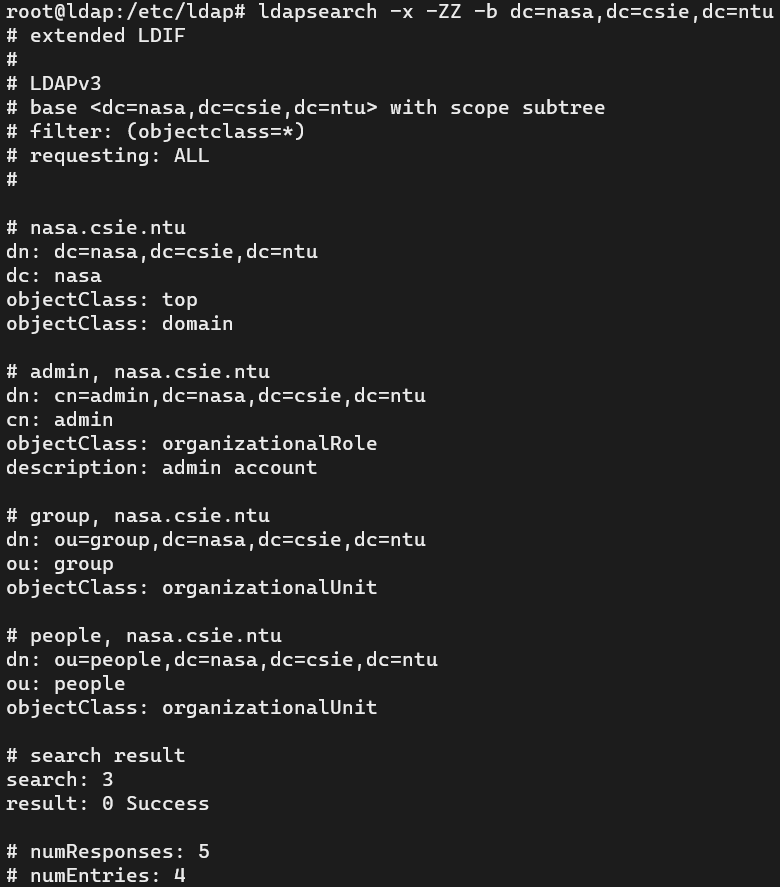
\includegraphics[width=0.8\textwidth]{1-b_ldapsearch_starttls.png}

    \begin{Verbatim}[frame=single]
$ ldapsearch -x -H ldaps:/// -b dc=nasa,dc=csie,dc=ntu
    \end{Verbatim}

    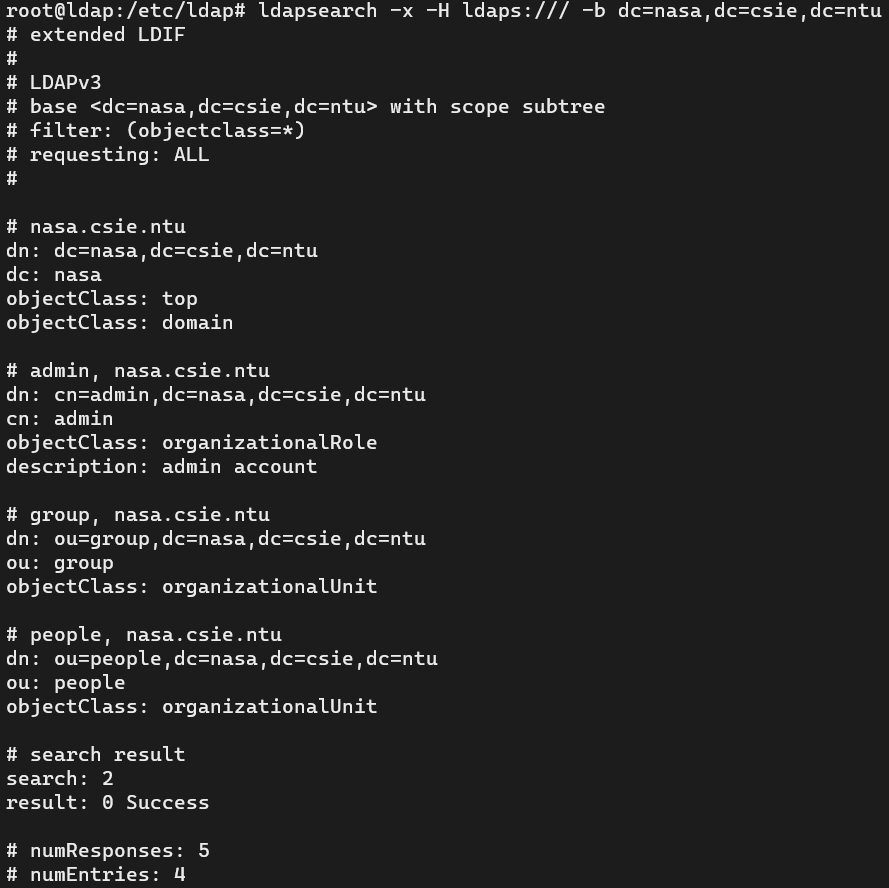
\includegraphics[width=0.8\textwidth]{1-b_ldapsearch_ldaps.png}
  \end{enumerate}

  \textbf{References}
  \begin{itemize}
    \item \href{https://www.openldap.org/doc/admin26/tls.html}{OpenLDAP Software 2.6 Administrator's Guide: Using TLS}
    \item \href{https://www.openldap.org/faq/data/cache/185.html}{OpenLDAP Faq-O-Matic: How do I use TLS/SSL?}
    \item \href{https://github.com/xbmc/openssl/blob/master/apps/CA.sh}{openssl/apps/CA.sh at master · xbmc/openssl · GitHub}
    \item \href{https://www.openssl.org/docs/man3.3/man1/openssl-ca.html}{/docs/man3.3/man1/openssl-ca.html}
    \item \href{https://www.openssl.org/docs/man3.3/man1/openssl-req.html}{/docs/man3.3/man1/openssl-req.html}
    \item \href{https://en.wikipedia.org/wiki/Certificate_signing_request}{Certificate signing request - Wikipedia}
    \item \href{https://www.openldap.org/doc/admin26/slapdconfig.html}{OpenLDAP Software 2.6 Administrator's Guide: The slapd Configuration File}
    \item \href{https://serverfault.com/questions/539226/how-to-enable-tls-on-openldap}{ssl - How to enable TLS on OpenLDAP - Server Fault}
    \item \href{https://stackoverflow.com/questions/51745010/ldap-modify-other-e-g-implementation-specific-error-80}{ldap - ldap\_modify: Other (e.g., implementation specific) error (80) - Stack Overflow}
    \item \href{https://www.linuxquestions.org/questions/linux-software-2/issues-with-openldap-and-ssl-tls-905840/}{[SOLVED] Issues with OpenLDAP and SSL / TLS}
    \item \href{https://www.linuxquestions.org/questions/linux-networking-3/ldap_start_tls-connect-error-11-a-497888/}{ldap\_start\_tls: Connect error (-11)}
    \item \verb|man slapd|, \verb|man slapd.conf|, and \verb|man slapd-config|
  \end{itemize}

  \pagebreak
  \section{Client setup}
  \begin{enumerate}[label=(\alph*)]
    \item \textbf{Steps}

    Install the \verb|openldap| package.
    \begin{Verbatim}[frame=single]
$ pacman -S openldap
    \end{Verbatim}

    \textbf{Result}
    \begin{Verbatim}[frame=single]
$ ldapsearch -x -H ldap://192.168.8.0 -b dc=nasa,dc=csie,dc=ntu
    \end{Verbatim}

    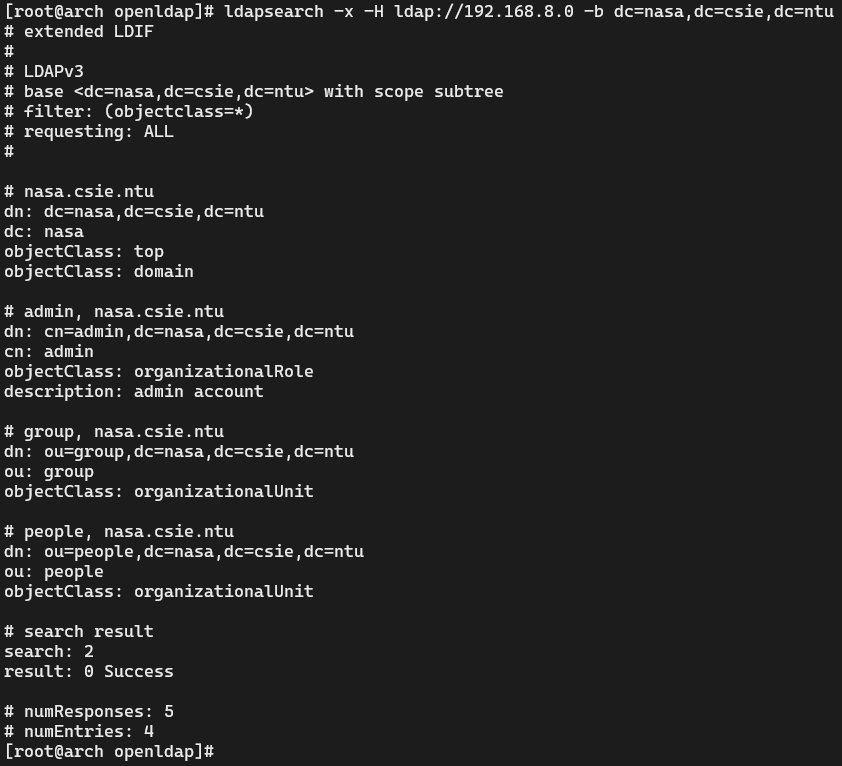
\includegraphics[width=0.8\textwidth]{2-a_ldapsearch.png}

    \textbf{References}
    \begin{itemize}
      \item \href{https://wiki.archlinux.org/title/openLDAP}{OpenLDAP - ArchWiki}
      \item \href{https://archlinux.org/packages/core/x86_64/openldap/}{Arch Linux - openldap 2.6.7-2 (x86\_64)}
    \end{itemize}

    \pagebreak
    \item \textbf{LDIF files}

    \verb|security.ldif|
    \inputminted{ldif}{ldif/security.ldif}

    \textbf{Steps}
    \begin{enumerate}[label=(\arabic*)]
      \item On the server configuration, set the \verb|olcSecurity| option to \verb|tls=1|.
      \begin{Verbatim}[frame=single]
$ ldapmodify -Y EXTERNAL -H ldapi:/// -f security.ldif
      \end{Verbatim}

      \item Set \verb|TLS_REQCERT allow| in the client's \verb|/etc/opneldap/ldap.conf|.
      This allows bad certificates (our certificate is self-signed) to be ignored, and the
      session proceeds normally.
      \begin{Verbatim}[frame=single]
# /etc/openldap/ldap.conf
TLS_REQCERT allow
      \end{Verbatim}
    \end{enumerate}

    \textbf{Result}
    \begin{Verbatim}[frame=single]
$ ldapsearch -x -H ldap://192.168.8.0 -b dc=nasa,dc=csie,dc=ntu
    \end{Verbatim}

    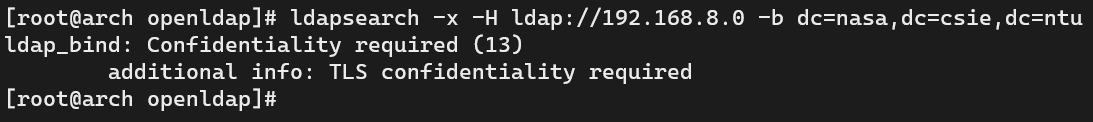
\includegraphics[width=0.93\textwidth]{2-b_ldapsearch_denied.png}

    \begin{Verbatim}[frame=single]
$ ldapsearch -ZZ -x -b dc=nasa,dc=csie,dc=ntu
$ ldapsearch -x -H ldaps:/// -b dc=nasa,dc=csie,dc=ntu
    \end{Verbatim}

    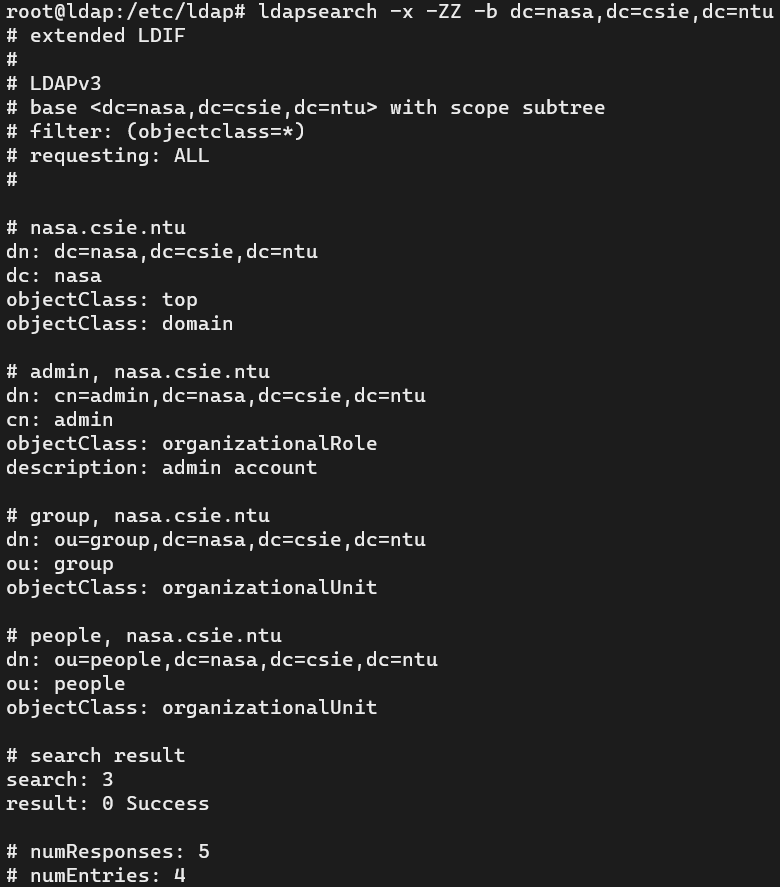
\includegraphics[width=0.46\textwidth]{1-b_ldapsearch_starttls.png}
    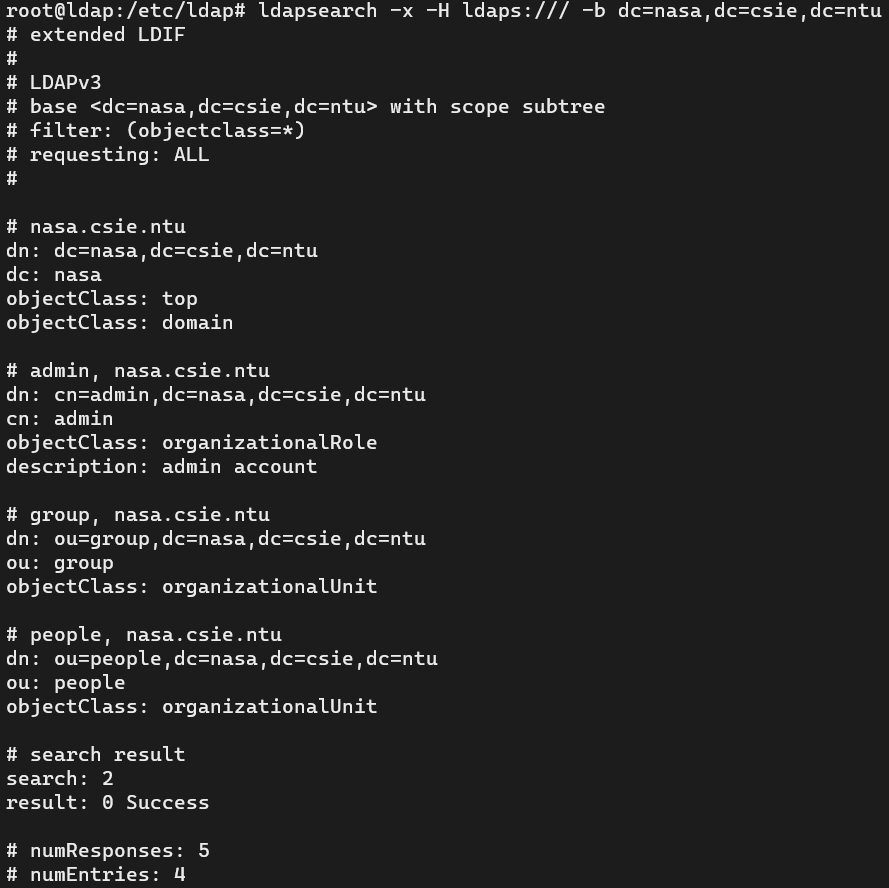
\includegraphics[width=0.46\textwidth]{1-b_ldapsearch_ldaps.png}

    \pagebreak
    \textbf{References}
    \begin{itemize}
      \item \href{https://wiki.archlinux.org/title/openLDAP#Start_slapd_with_SSL}{OpenLDAP - ArchWiki (2.5.3 Start slapd with SSL)}
      \item \href{https://serverfault.com/questions/459718/configure-openldap-with-tls-required}{ldap - Configure OpenLDAP with TLS=required - Server Fault}
      \item \verb|man ladp.conf| and \verb|man slapd-config|
    \end{itemize}

    \item \textbf{Steps}
    \begin{enumerate}[label=(\arabic*)]
      \item Install the \verb|sssd| and \verb|sudo| packages.
      \begin{Verbatim}[frame=single]
$ pacman -S sssd sudo
      \end{Verbatim}

      \item Edit \verb|/etc/sssd/sssd.conf| to the following configuration.
      \begin{Verbatim}[frame=single, fontsize=\footnotesize]
#/etc/sssd/sssd.conf
[sssd]
config_file_version = 2
services = nss, pam, sudo
domains = LDAP

[domain/LDAP]
cache_credentials = true
enumerate = true
id_provider = ldap
auth_provider = ldap
ldap_uri = ldap://192.168.8.0
ldap_search_base = dc=nasa,dc=csie,dc=ntu
ldap_id_use_start_tls = true
ldap_tls_reqcert = allow
chpass_provider = ldap
ldap_chpass_uri = ldap://192.168.8.0
      \end{Verbatim}
      \item Change permission of \verb|/etc/sssd/sssd.conf| to 600.
      \begin{Verbatim}[frame=single]
$ chmod 600 /etc/sssd/sssd.conf
      \end{Verbatim}

      \item Edit the following options in  \verb|/etc/nsswitch.conf|.
      \begin{Verbatim}[frame=single, fontsize=\footnotesize]
#/etc/nsswitch.conf
passwd: files systemd sss
group: files [SUCCESS=merge] systemd sss
shadow: files systemd sss
gshadow: files systemd sss
sudoers: files sss

...
      \end{Verbatim}

      \pagebreak
      \item Add the following lines to \verb|/etc/pam.d/system-auth|.
      \begin{Verbatim}[frame=single, fontsize=\footnotesize, breaklines]
#/etc/pam.d/system-auth
auth sufficient pam_sss.so forward_pass
auth required pam_faillock.so preauth

...

account [default=bad success=ok user_unknown=ignore authinfo_unavail=ignore] pam_sss.so
-account [success=1 default=ignore] pam_systemd_home.so

...

password sufficient pam_sss.so

...

session required pam_mkhomedir.so skel=/etc/skel/ umask=0077
-session optional pam_systemd_home.so
session required pam_limits.so
session required pam_unix.so
session optional pam_sss.so
      \end{Verbatim}

      \item \verb|/etc/pam.d/sudo| includes \verb|system-auth| by default, so
      we don't need to make manual changes.

      \item Restart services.
      \begin{Verbatim}[frame=single]
$ systemctl sssd.service sshd.service
      \end{Verbatim}
    \end{enumerate}

    \textbf{References}
    \begin{itemize}
      \item \href{https://en.wikipedia.org/wiki/System_Security_Services_Daemon}{System Security Services Daemon - Wikipedia}
      \item \href{https://wiki.archlinux.org/title/LDAP_authentication#Online_and_offline_authentication_with_SSSD}{LDAP authentication - ArchWiki (2.2 Online and offline authentication with SSSD)}
      \item \href{https://man.archlinux.org/man/sssd.conf.5}{sssd.conf(5) — Arch manual pages}
      \item \href{https://man.archlinux.org/man/sssd-ldap.5.en}{sssd-ldap(5) — Arch manual pages}
      \item \href{https://linux.die.net/man/5/nsswitch.conf}{nsswitch.conf(5) - Linux man page}
      \item \href{https://linux.die.net/man/5/pam.d}{pam.d(5) - Linux man page}
    \end{itemize}

    \pagebreak
    \item \textbf{LDIF files}

    \verb|groups.ldif|
    \inputminted[fontsize=\footnotesize]{ldif}{ldif/groups.ldif}

    \verb|users.ldif|
    \inputminted[fontsize=\footnotesize]{ldif}{ldif/users.ldif}

    \verb|sudoers.ldif|
    \inputminted[fontsize=\footnotesize]{ldif}{ldif/sudoers.ldif}

    \textbf{Steps}
    \begin{enumerate}[label=(\arabic*)]
      \item Temporarily disable \verb|olcSecurity|, then add the sudo schema.
      \begin{Verbatim}[frame=single, fontsize=\footnotesize]
$ wget https://github.com/sudo-project/sudo/raw/main/docs/schema.olcSudo
$ ldapadd -Y EXTERNAL -H ldapi:/// -f schema.olcSudo
      \end{Verbatim}
      \item Add the groups, users, and sudoers records.
      \begin{Verbatim}[frame=single, fontsize=\footnotesize]
$ ldapadd -Z -D cn=admin,dc=nasa,dc=csie,dc=ntu -w admin -H ldapi:/// \
    -f groups.ldif
$ ldapadd -Z -D cn=admin,dc=nasa,dc=csie,dc=ntu -w admin -H ldapi:/// \
    -f users.ldif
$ ldapadd -Z -D cn=admin,dc=nasa,dc=csie,dc=ntu -w admin -H ldapi:/// \
    -f sudoers.ldif
      \end{Verbatim}
    \end{enumerate}

    \textbf{Result}
    \begin{Verbatim}[frame=single]
[root@arch /]# ssh b12902110@localhost
b12902110@localhost's password:
Creating directory '/home/b12902110'.
[b12902110@arch ~]$ sudo echo Hello World
[sudo] password for b12902110:
b12902110 is not allowed to run sudo on arch.

[root@arch /]# ssh ta1@localhost
ta1@localhost's password:
Creating directory '/home/ta1'.
[ta1@arch ~]$ sudo echo Hello World
[sudo] password for ta1:
Hello World
    \end{Verbatim}

    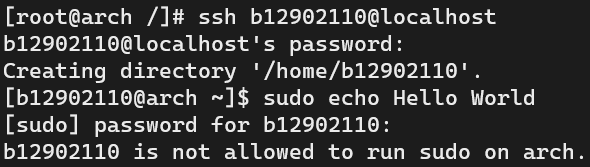
\includegraphics[width=0.6\textwidth]{2-d_b12902110.png}

    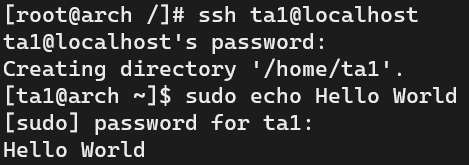
\includegraphics[width=0.5\textwidth]{2-d_ta1.png}

    \textbf{References}
    \begin{itemize}
      \item \verb|ws5:~$ ldapsearch -x cn=student|
      \item \href{https://www.sudo.ws/docs/man/1.8.17/sudoers.ldap.man/}{Sudoers LDAP Manual | Sudo}
      \item \href{https://www.sudo.ws/docs/readme/readme_ldap/}{README.LDAP | Sudo}
      \item \href{https://github.com/sudo-project/sudo/blob/main/docs/schema.olcSudo}{sudo/docs/schema.olcSudo at main · sudo-project/sudo · GitHub}
    \end{itemize}
  \end{enumerate}

  \section{Access Control Lists}
  \textbf{LDIF files}

  \verb|acl.ldif|
  \inputminted{ldif}{ldif/acl.ldif}

  \textbf{Steps}

  Temporarily disable \verb|olcSecurity|, then commit \verb|ACL.ldif|.
  \begin{Verbatim}[frame=single]
$ ldapmodify -Y EXTERNAL -H ldapi:/// -f acl.ldif
  \end{Verbatim}

  \textbf{Result}
  \begin{enumerate}[label=(\alph*)]
    \item Users can only change its own information, and cannot change other users'
    information.

    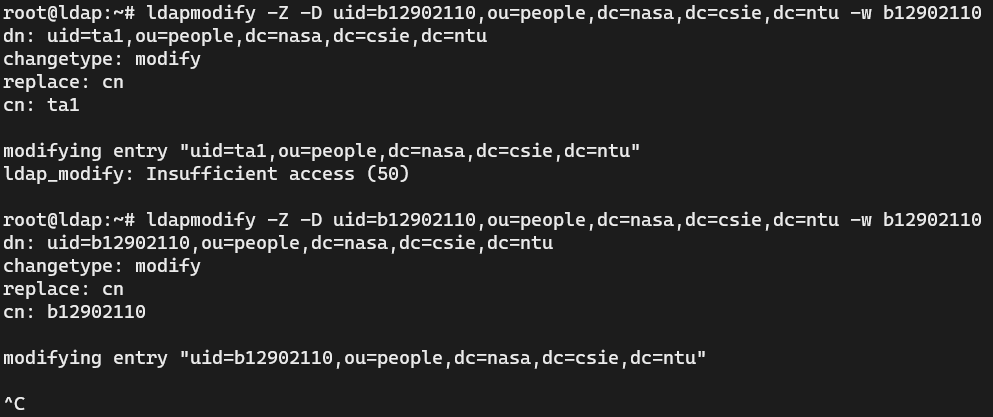
\includegraphics[width=0.9\textwidth]{3-a_ldapmodify.png}

    \item Users cannot change UID, GID and home directory.

    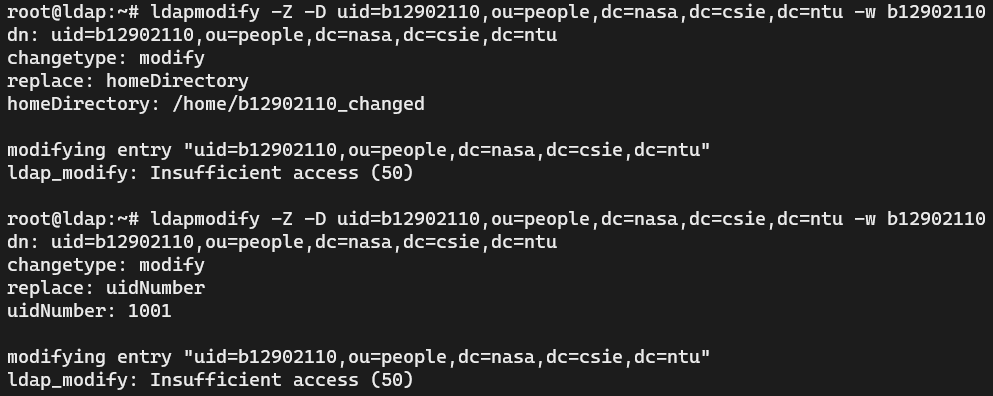
\includegraphics[width=0.9\textwidth]{3-b_ldapmodify.png}

    \item Anonymous can read information except password.

    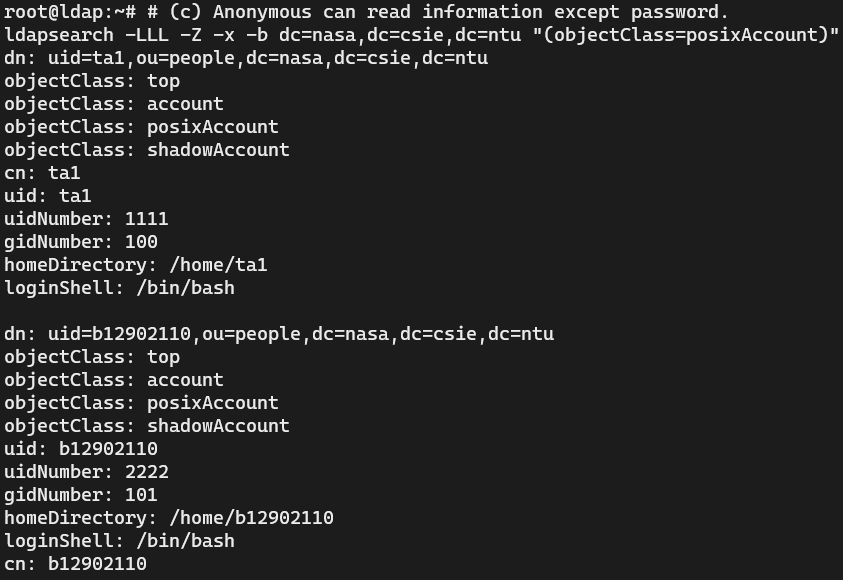
\includegraphics[width=0.9\textwidth]{3-c_ldapsearch.png}
  \end{enumerate}

  \textbf{References}
  \begin{itemize}
    \item \href{https://www.openldap.org/doc/admin26/access-control.html}{OpenLDAP Software 2.6 Administrator's Guide: Access Control}
    \item \href{https://serverfault.com/questions/537737/how-to-correctly-ldapmodify-replace-olcaccess-lines}{debian - How to correctly ldapmodify replace olcAccess lines? - Server Fault}
  \end{itemize}

  \pagebreak
  \section{Scripts}

  The scripts should be run at the server since we're using \verb|-H ldapi:///|.\\

  \verb|add_user.sh|
  \inputminted[fontsize=\footnotesize]{shell}{scripts/add_user.sh}

  \pagebreak
  \verb|del_user.sh|
  \inputminted[fontsize=\footnotesize]{shell}{scripts/del_user.sh}

  \textbf{Result}
  \begin{Verbatim}[frame=single]
$ ./add_user.sh
Admin password (password for cn=admin,dc=nasa,dc=csie,dc=ntu):
Username: user1
Password:

...

adding new entry "uid=user1,ou=people,dc=nasa,dc=csie,dc=ntu"

$ ldapsearch -LLL -x -b dc=nasa,dc=csie,dc=ntu uid=user1
dn: uid=user1,ou=people,dc=nasa,dc=csie,dc=ntu
objectClass: top
objectClass: account
objectClass: posixAccount
objectClass: shadowAccount
cn: user1
uid: user1
uidNumber: 2223
gidNumber: 101
homeDirectory: /home/user1
loginShell: /bin/bash

$ ./del_user.sh
Admin password (password for cn=admin,dc=nasa,dc=csie,dc=ntu):
Username: user1

Deleting user user1...
dn: uid=user1,ou=people,dc=nasa,dc=csie,dc=ntu

$ ldapsearch -LLL -x -b dc=nasa,dc=csie,dc=ntu uid=user1
  \end{Verbatim}

  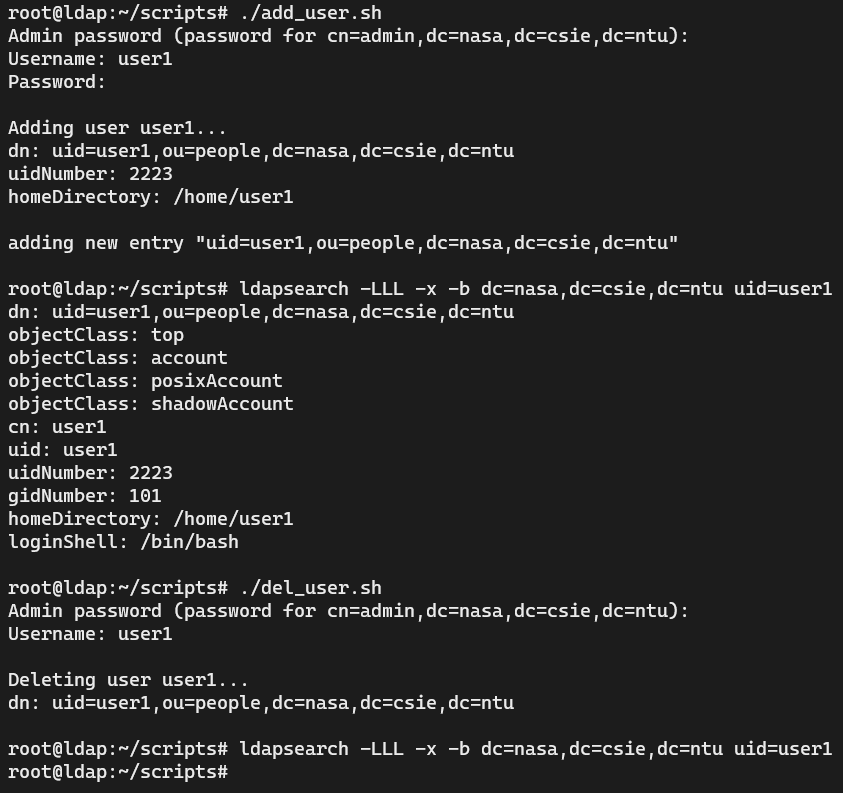
\includegraphics[width=0.9\textwidth]{4_result.png}

  \textbf{References}
  \begin{itemize}
    \item \href{https://systemd.io/UIDS-GIDS/}{Users, Groups, UIDs and GIDs on systemd Systems}
    \item \href{https://stackoverflow.com/questions/18544359/how-do-i-read-user-input-into-a-variable-in-bash}{shell - How do I read user input into a variable in Bash? - Stack Overflow}
    \item \href{https://www.gnu.org/software/bash/manual/html_node/Bash-Builtins.html#index-read}{Bash Builtins (Bash Reference Manual) (read)}
    \item \href{https://www.gnu.org/software/bash/manual/html_node/Redirections.html#Here-Documents}{Redirections (Bash Reference Manual) (3.6.6 Here Documents)}
    \item \href{https://www.openldap.org/software/man.cgi?query=slappasswd&apropos=0&sektion=0&manpath=OpenLDAP+2.6-Release&arch=default&format=html}{slappasswd}
    \item \href{https://www.openldap.org/software/man.cgi?query=ldapdelete&apropos=0&sektion=0&manpath=OpenLDAP+2.6-Release&arch=default&format=html}{ldapdelete}
  \end{itemize}

\end{document}
